\chapter{Технологический раздел}

\section{Выбор и обоснование языка программирования}

Для разработки программного комплекса был выбран язык C++ и среда разработки Qt 4.8. Данная среда является кроссплатформеной и обладает огромной библиотекой классов, что существенно упрощает разработку. Для перенесения программы на другую операционную систему требуется лишь ее перекомпиляция. Язык C++ является мощнейшим инструментом разработки: он имеет строгую типизацию и объектно-ориентирован, обеспечивает возможность быстрой разработки приложений, но при этом сохраняет выразительность и элегантность.

\section{Структура программного комплекса}

Внутреннее строение системы имеет модульную структуру, и каждый модуль отвечает за определенные функции. Все модули и классы, реализованные в нем, можно разделить на два типа:
\begin{itemize}
\item классы, реализующие интерфейс программы;
\item классы, отвечающие за логику работы.
\end{itemize}

Было принято решение не выделять отдельной сущностью менеджера, т.к. система имеет практически линейный сценарий и к ней не предъявляются требования по сохранению собственного состояния. Вся нагрузка по взаимодействию элементов ложится на класс главной формы. Стоит отметить, что реакция системы на неверные входные данные реализована в виде негативного результата функции, т.к. механизм исключений \textit{try} ... \textit{catch} не имеет должной поддержки в Qt из-за особенностей реализации фреймворка.

На вход системе поступает XMI-файл, содержащий описание диаграммы. Разбор и построение списка состояний и переходов диаграммы производится в методе \textit{parse} класса \textit{XMLEngine} . Исходя из особенностей структуры XMI разбор файла производится вручную. Для этого, перед основной функцией разбора вызывается метод \textit{validate} класса \textit{XMLValidator}, который проверяет соответствие структуры файла xml-схеме (см. \ref{cha:appendix1}). В ходе разбора сначала заполняется список состояний диаграммы \textit{states}, а потом, основываясь на этом списке строиться список переходов \textit{transitions}. Каждое состояние имеет свой уникальный id, по которому происходит связывание текущего перехода transition с исходной и целевой вершиной.

В случае удачного разбора файла происходит отображение диаграммы. Для большей гибкости приложения, само отображение диаграммы на плоскости вынесено в отдельный класс и для визуализации используется паттерн посетитель. Парадигма ядра графического движка Qt основана на представлении отдельных примитивов как объектов и дальнейшим их позиционировании на плоскости.

Каждый потомок абстрактного класса \textit{State} имеет переопределенный метод \textit{diagramItem()}, который создает соответствующий класс, наследуемый от абстрактного \textit{QGraphicsItem}, и отвечающий за отображение этого типа элемента диаграммы.

Диаграмма классов представлена на рисунке \ref{fig:fig20}.

\begin{figure}
	\begin{center}
		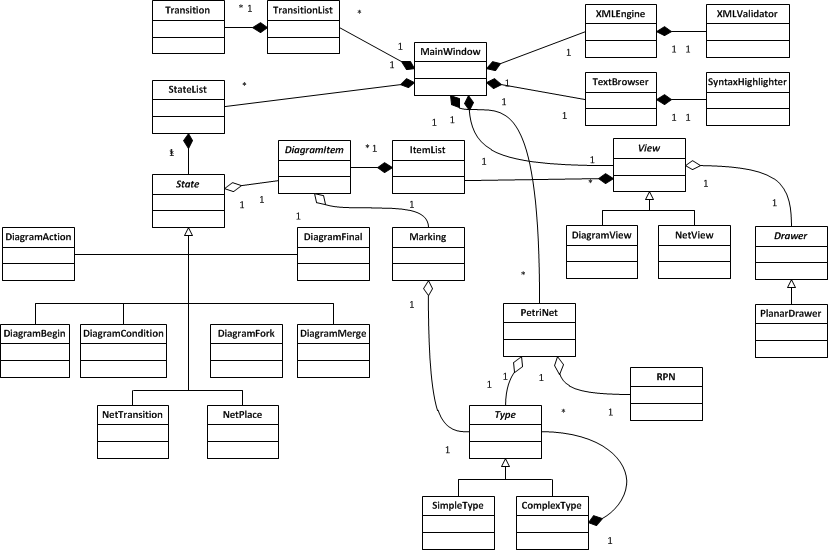
\includegraphics[width=\textwidth]{include/ClassDiagram.png}
	\end{center}
	\caption{Диаграмма классов системы}
	\label{fig:fig20}
\end{figure}

\section{Реализация алгоритмов работы системы}

\subsection{Построение списка переменных}

Для преобразования в раскрашенную сеть Петри необходимо иметь информацию о переменных, используемых диаграммой. Переменные могут фигурировать в диаграмме в блоках действий или в спусковых функциях переходов. Для разбора переменных будем использовать алгоритм поиска в глубину. Структура данных для описания типов приведена на рисунке \ref{fig:fig21}.

\begin{figure}
	\begin{center}
		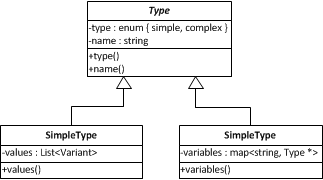
\includegraphics[scale=1]{include/Type.png}
	\end{center}
	\caption{Структура классов для описания типов переменных.}
	\label{fig:fig21}
\end{figure}

Все переменные можно разделить условно на два типа: простые и составные (структурные). Для простых переменных в классе SimpleType используется список сериализованных данных \textit{list<variant>}. Структурный тип, реализованный классом ComplexType, имеет именованный список переменных \textit{map<string, type *>}.	

\subsection{Преобразование в простую сеть Петри}

Каждый элемент диаграммы преобразуется в позиции и переходы таким образом, что позиции соединены с переходами, но они не имеют входных дуг, а переходы выходных. Исключения составляют начальное и конечное состояние. Начальное состояние имеет только одну выходную дугу, а значит мы можем его вообще не учитывать, а выходной переход преобразуется только в соответствующую позицию. Так как ограничения переходов могут накладываться только на блок условного перехода, при преобразовании условие преобразуется в спусковую функцию внутренней дуги между позицией и переходом.
Алгоритм преобразования состоит из двух частей:
\begin{itemize}
\item преобразование каждого элемента диаграммы в соответствующий набор позиций и переходов сети;
\item связывание преобразовыванных элементов друг с другом.
\end{itemize}

Позиции и переходы являются наследниками абстрактного класса \textit{State}, а значит для их идентификации используется поле \textit{id}. Для каждой позиции идентификатор формируется как \textit{id} преобразовываемого элемента, метка \textit{place} и порядковый номер, если позиций больше одной. Аналогично для переходов. Из-за этого нарушается четкая взаимосвязь между состояниями и переходами сети, т.е. после первого этапа преобразования нельзя четко сказать какая дуга из  перехода в позицию будет соответствовать дуге в исходном описании. Необходимо реализовать связь элементов сети, производя поиск незанятых позиций и переходов.
\begin{lstlisting}[style=pseudocode,caption={Алгоритм преобразования в простую сеть Петри}]
queue << states.find(begin)
while !queue.empty():
	State * state = queue.takeFirst()
	if !netStates->find(state->id()):
		convertState(state)
	foreach transition in state.outgoing:
		if !netStates->find(target->id()):
			queue.append(target)
			convertState(target)
		if state->type() != begin_state:
			State * transition, * place;
			List<State *> transitions = netStates->find(state->id() + "transition")
			if state->type() = condition_state:
				transition = findFreeTransition(transitions)
			else
				transition = transitions.first()
			List<State *> places = netStates->find(target->id() +  "place");
			if target->type() == merge_state:
				place = findFreePlace(places)
			else
				place = places.first()
			Transition * tr = new Transition(state->id() + "-" + target->id())
\end{lstlisting}

\subsection{Формирование множества активных переходов}

В процессе моделирования на каждом шаге возникает задача поиска множества активных переходов. Для решения этой задачи можно последовать двумя путями:

\begin{itemize}
\item поиск всех переходов и выделение списка активных переходов;
\item поиск всех позиций, содержащих фишки, и на основании этого построение списка возможных переходов.
\end{itemize}

Так как каждая позиция может иметь несколько исходящих переходов, а каждый переход может иметь несколько входных позиций, задача определения множества активных переходов в общем случае сводится к полному перебору. С учетом специфики преобразования диаграммы, получаем, что из одной позиции может быть несколько переходов только в случае условного перехода и все исходящие переходы для этой позиции имеют лишь одну входящую дугу. Переход может иметь несколько входных позиций только в случае слияния, а значит, все позиции имеют лишь одну исходящую дугу. Для всех остальных случаев каждый переход имеет лишь одну входную дугу, а каждая позиция лишь одну исходящую.

Основываясь на этом, опишем алгоритм формирования множества активных переходов:
\begin{lstlisting}[style=pseudocode,caption={Алгоритм формирования множества активных переходов}]
List<Place *> list, places = states->find(place)
MultiMap<Place *, Transition *> activeTransitions
foreach place in places:
	if place->marking > 0:
		list.append(place)
foreach transition in place->outgoing:
	bool flag = true
	foreach place in transition->incoming:
		if place->marking = 0 and calculate(transition->guard, place->marking):
			flag = false	
	if flag:
		activeTransitions.insert(place, transition)
\end{lstlisting}

\section{Формирование раскраски сети}

Задача формирования раскраски сети состоит из двух этапов:
\begin{itemize}
\item выделение множества цветов на основе используемых переменных;
\item определение максимальной области видимости переменных.
\end{itemize}

Алгоритм опеределения максимальной области видимости переменных реализуется поискомв глубину. Список \textit{track} хранит путь из корня до текущей вершины. Основаная идея алгоритма заключается в том, что если мы для некоторой позции список переменных содержит искомую переменную, то добавляем эту переменную для всех просмотренных вершин из текущей до предыдущей вершины, содержащей эту переменную.

\begin{lstlisting}[style=pseudocode,caption={Алгоритм опеределения максимальной области видимости переменных}]
def path(state, variable, track):
    foreach transition in state->outgoing:
        Place * place = transition->target()
        if variable in place->variables():
            foreach state in track:
                if state->type = place and variable in state->varibles():
                    foreach place from current state to track.last():
                        place->variables << variable
        if target not in track:
            track << target
            path(target, variable, track);
            track remove last
\end{lstlisting}

\section{Анализ работоспособности программного комплекса}

Рассмотрим базовые элементы UML диаграмм деятельности в аспекте их отражения на элементарную базу сетей Петри. 

Пусть имеется квадратное поле 3х3, каждая клетка которого условно содержит некоторое количество ресурсов. На одной из клеток изначально находится игрок, способный перемещаться за один ход на одну клетку в любую сторону (рис. \ref{fig:fig27}).

\begin{figure}
	\begin{center}
		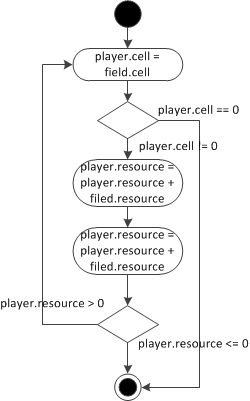
\includegraphics[scale=1]{include/ActivityDiagram.png}
	\end{center}
	\caption{Диаграмма деятельности, представляющая алгоритм решения поставленной задачи.}
	\label{fig:fig27}
\end{figure}

Цикл работы данной симуляции состоит из следующих шагов:
\begin{enumerate}
\item[1.] выбор смежной клетки, которая еще не была посещена. Если таковых не осталось, игра заканчивается, иначе переход к пункту 2;
\item[2.] перемещение в выбранную клетку;
\item[3.] ресурсы, сопоставленные с этой клеткой, становящиеся достоянием игрока, т. е. прибавляемые к некоторому счетчику, изначально нулевому. Однако на перемещение затрачивается некоторое фиксированное количество ресурсов. Если суммарное накопление ресурсов стало отрицательным, игрок не может продолжать движение и игра останавливается.
\end{enumerate}

Для анализа рабоспособности метода проведем сравнение результатов моделирования задачи с помощью разработанного метода и моделирующей программы CPN Tools.

Раскрашенная сеть Петри, построенная в среде CPN Tools, приведена на рисунке \ref{fig:fig28}.

\begin{figure}
	\begin{center}
		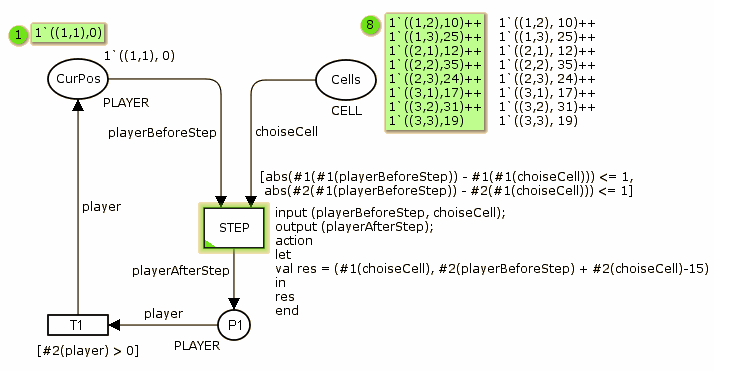
\includegraphics[scale=1]{include/CPNTools.png}
	\end{center}
	\caption{Раскрашенная сеть Петри в CPN Tools.}
	\label{fig:fig28}
\end{figure}

Для обработки модели в CPN Tools вводятся следующие типы данных:

\begin{verbatim}
colset POSITION = product INT * INT
colset PRICE = INT
colset CELL = PRODUCT POSITION * PRICE
colset PLAYER = product POSITION * PRICE
\end{verbatim}

Тип POSITION обозначает пару целых чисел, предназначенных для обозначения номера строки и столбца клетки, тип PRICE ~--- целое значение количества ресурсов клетки, тип CELL обозначает клетку и включает в себя позицию и цену, тип PLAYER введен для обозначения игрока и хранит в себе его текущие позицию и количество собранных ресурсов. На следующем этапе объявляются дуговые переменные:
\begin{verbatim}
playerBeforeStep, playerAfterStep, player : PLAYER
choiseCell : CELL
\end{verbatim}

В curPos заданы начальный маркер, обозначающий игрока в позиции (1;1), и обнуленный счетчик накопленных ресурсов. В позиции Cells определено восемь маркеров, соответствующих прочим клеткам игрового квадрата, каждая клетка представлена своими координатами и предопределенным уровнем ресурсов. Переход STEP обозначает действие: выбор смежной клетки и получения ее ресурсов. Для данного перехода задано следующее условие срабатывания:

\begin{verbatim}
[abs(#1(#1(playerBeforeStep)) - #1(#1(choiceCell))) <= 1
 abs(#2(#1(playerBeforeStep)) - #2(#1(choiceCell))) <= 1]
\end{verbatim}

Конструкция #1(x) означает «взять первый элемент в x». Таким образом, условие осуществляет проверку: следующая клетка, выбранная для перемещения, смежная с текущей позицией игрока. Благодаря этому условию игрок перемещается в случайном порядке, за один ход преодолевая один квадрат. После каждого хода количество маркеров в позиции Cells уменьшается на единицу, поскольку переход STEP их изымает. Это соответствует тому, что уже посещенные клетки недоступны для перемещения.
Переход STEP содержит следующую подпрограмму:

\begin{verbatim}
input(playerBeforeStep, choiseCell);
output(playerAfterStep);
action
    let
    val res = (#1(choiseCell), #2(playerBeforeStep) +
    + #2(choiseCell) - 1)
    in
    res
end
\end{verbatim}

Здесь описаны входные (игрок и доступная клетка) и выходные параметры (игрок, совершивший ход). Алгоритм подпрограммы прост: в маркер игрока записывается позиция выбранной клетки, а к его счетчику ресурсов добавляется количество ресурсов этой клетки и вычитается 15 (число, взятое за цену перемещений).

Стоит отметить, что не каждая из возможных последовательность выбора следующей клетки при оговоренных ограничениях приведет к посещению всех клеток. Симуляция сети Петри в CPN Tools позволяет построить пространство возможных состояний и увидеть, какие ходы оптимальны, какая стратегия выбора более выигрышная.

При преобразовании диаграммы с помощью разработанного метода автоматически выделяется список переменных для каждого состояния, и у пользователя запрашивается ввод их исходных значений:

\begin{verbatim}
player : struct { cell, resource } = [ ((1, 1), 0) ]
field : struct { cell, resource } =
[ ((1, 2), 10); ((1, 3), 25); ((2, 1), 12); ((2, 2), 35);
  ((2, 3), 24); ((3, 1), 17); ((3, 2), 31); ((3, 3), 19) ]
resource : simple type = 15
\end{verbatim}

На основе алгоритма опеределения максимальной области видимости переменных строится результирующая раскраска графа (рис. \ref{fig:fig29})

\begin{figure}
	\begin{center}
		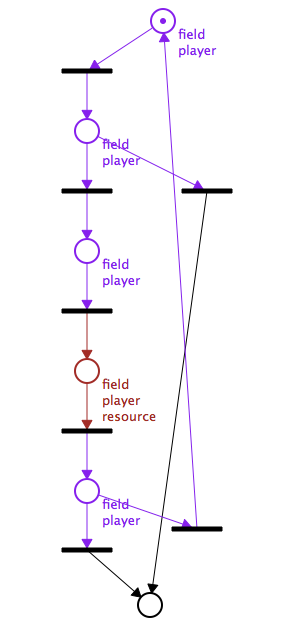
\includegraphics[scale=1]{include/PetriNet.png}
	\end{center}
	\caption{Раскрашенная сеть Петри, полученная с помощью разработнного метода.}
	\label{fig:fig29}
\end{figure}

В процессе моделирования мы получаем, что фишка приходит в конечное состояние и все фишки сети были использованы. Это означает отсустствие блокировок и недостижимых состояний сети, а значит корректность исходных данных для поставленной задачи.

В отличии от CPN Tools, где построением сети занимается пользователь, разработнная система выстраивает сеть автоматически, для этого лишь требуется полное описание диаграммы деятельности и начальные значения переменных.

\label{cha:implementation}

